\documentclass{article}

\usepackage[spanish]{babel}
\usepackage[numbers,sort&compress]{natbib}
\usepackage[T1]{fontenc}
\usepackage[ansinew]{inputenc}
\usepackage{graphicx}
\usepackage{url}

\title{Pr\'actica 2: Aut\'omata Celular}
\author{Anahi Llano}
\begin{document}
\maketitle

\section{Introducci\'{o}n}\label{into}

Se realiza la segunda p\'ractica \cite{elisa} llamada aut\'omata celular.
 
\section{Metodolog\'{i}a}\label{met}

Se tomo en cuenta las indicaciones dadas en la p\'{a}gina de la clase \cite{elisa}, realizando ya sea la opci\'on a) El mayor colapso poblacional o el b) El mayor tiempo continuo de vida en una celda tomando como ejemplo el repositorio \cite{SatuElisa} modificando el c\'odigo para obtener alguna de las opciones anteriores.

\section{Resultados y Discusi\'{o}n}\label{res}

Una vez modificado el c\'odigo y mediante un an\'alisis se pueden observar ambas opciones.
a) Para el mayor colapso poblacional, se modific\'o el c\'odigo de tal manera que dijera en cada iteraccion cuantos vivos se obtuvieron. \cite{ana} el extracto de datos se puede observar en el archivo "vivosxiteracion" que se encuentra en el repositorio.

\begin{table}
  \caption{Vivos por iteraci\'on}
  \label{t1}
  \begin{center}
    \begin{tabular}{rrr}
      iteracion & \texttt{vivos}
      0 &  93        \\
      1 &  63        \\
      2 &  34       \\
      3 &  26    \\
      4 &  21  \\
      5 &  15 \\
      6 &  12 \\ 
      7 &  8   \\
      8 &  6  \\
      9 &  4  \\
      50 &  4  

\end{tabular}
\end{center}
\end{table}
  
En la tabla \ref{t1} se muestra el total de vivos por cada iteracion, se observa que a partir de la iteracion 9 se mantiene estable y son 4 vivos continuos hasta obtener las 50 repeticiones, por lo tanto, seg\'un se observa en la tabla \ref{t1} el mayor colapso poblacional fue de 30 celdas que ocurri\'o al pasar del tiempo 0 al tiempo 1.

Por otra parte, para obtener el mayor tiempo de vida igual se realiz\'o una modificaci\'on para mapear las posiciones de los vivos, mandarlos a un text y de ah\'i una gr\'afica donde se observan en que posiciones se encuentran los que m\'as se repitieron.

\begin{figure}
  \begin{center}
    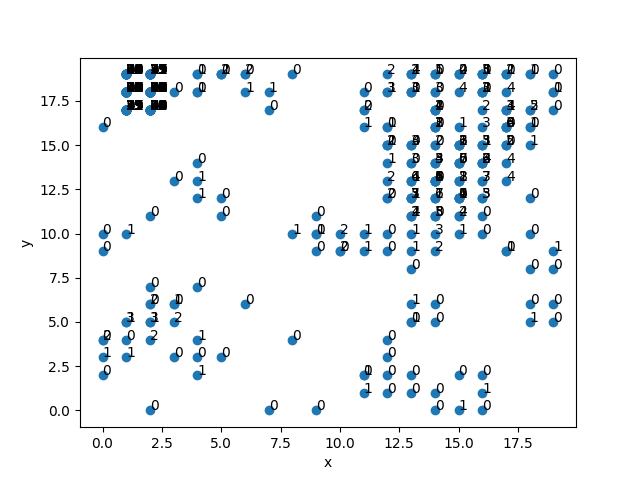
\includegraphics[width=10cm]{posiciones.png}
  \end{center}
  \caption{Mapeo de vivos.}
  \label{f1}
\end{figure}

Mapeando los lugares donde se observa m\'as negro se muestran las celdas que m\'as tiempo de vida tuvieron, y para confirmar cuantas itertaciones duraron se observ\'o con una b\'usqueda a partir del documento de tex \cite{ana} titulado "mapeovivos" que tambien se encuentra en el repositorio.

\begin{table}
  \caption{Mapeo de vivos.}
  \label{t2}
  \begin{center}
    \begin{tabular}{rrr}
      Fila & \texttt{Columna} & \texttt{Iteraciones que vivio} \\
      2 &  17    & 50     \\
      2  &  18   &  26    \\
      2  &  19    & 25   
    \end{tabular}
    \end{center}
  \end{table}
Seg\'un la tabla \ref{t2} que es un extracto de algunos datos que m\'as se repet\'ian se observa que la celda ubicada en el 2,17 fue la que obtuvo mayor tiempo de vida.
Para observar c\'omo se llevaron a cabo las iteraciones se muestra la imagen \cite{ana} "gameover" tambi\'en presente en el repositorio.

\section{Reto1}\label{ret}

Para el reto 1 se modific\'o el c\'odigo para simular el crecimiento de grano grueso y obtener la figura en 2D basado en el art\'iculo \cite{ret1} en donde se tom\'o como inspiraci\'on la ecuaci\'on diferencial para modificar la regla del aut\'omata celular. cabe mencionar que en el gif obtenido \cite{ana1} para que se pueda observar una diferencia significativa ser\'ia mejor probarlo con un mayor n\'umero de repeticiones, por motivos del procesador en la computadora no se pudo correr m\'as veces.

\section{Reto2}\label{reto}

para el reto 2 de igual manera se modific\'o el c\'odigo para obtener una figura en 3D, modificando la regla del aut\'omata en este caso no se corrio el c\'odigo ya que ser\'ia pesado para la computadora con la cual se trabaj\'o.

  \section{Conclusi\'{o}n}\label{con}
 Al cambiar la probabilidad inicial de una celda viva conforme al n\'umero de repeticiones, dif\'icilmente puede aumentar el n\'umero de celdas vivas.
El mayor colapso se da en la primera iteracion, y en este caso el mayor tiempo continuo es m\'as f\'acil observar cuando se cumplen las 50 repeticiones.

  \bibliography{refes}
  \bibliographystyle{plainnat}
\end{document}